%% A 3-page report (5 points) that:
% 1. Clearly documents the representations (variables, domains and constraints)
% that you devised for solving nonograms.
% 2. Explains the heuristics used for this problem. Note that heuristics appear 
% in at least two places in A*-GSP: a) in A*’s traditional h function, and b) 
% in the choice of a variable on which to base the next assumption. Both (and 
% others, if relevant) should be mentioned in the report.
% 3. Briefly overviews the primary subclasses and methods needed to specialize 
% your general-purpose A*-GAC system to handle nonograms.
% 4. Mentions any other design decisions that are, in your mind, critical to 
% getting the system to perform well.

\section{Central aspects of the Nonogram implementation}
This report describes our implementation and solution to given nonogram problem.

\subsection{Variables, domains, constraints}
For our representation of a Nonogram we have chosen to
use the rows and columns as variables. An idealized pseudocode
version can be seen below. The domain of each variable consists
of all the possible permutations of strings where 1 represents
\emph{marked} and 0 represents \emph{unmarked} in the final Nonogram.

If the amount of columns is 5, and a row has the set of segment
sizes \(\{1, 2\}\) our generated domains for this row, \(rn\), will be
\([`10110', `01011', `10011']\).

As shown in the code below, we will do lookup in these strings
crosschecked with a column in cell c, to check whether the constraint
is satisfied. This is similiar to what the module text describes in
\emph{2.2 Using an Aggregate Representation} and shows in Figure 3.

As an example if \(rn\) above was \(r1\) (zero-indexed), and we had a column
\(c3\), we can clearly see from the example that \(c3[1]\) must be 1, as all the
valid domains for \(r1\) contain 1 at the fourth position. So given domains
for \(domains[c3] = [`1010', `1100', `0011']\), our implementation of revise
would limit the domain of \(c3\) to \([`1100']\).

\lstinputlisting[emph={Nonogram},label={code:nonogram},caption={Generating the variables and constraints.}]{module_3/code_snippets/nonogram.py}

\subsection{Heuristics}
The heuristics is equal to the heuristics of module 2, but since the reports is independent of each other, we have chosen to include the same description of the heuristics here as well.

Here, as in module 2, it's two heuristics at play, one that selects the successors and one that determines which node to get expanded first. For the selection of successors, we simply select the variable that has the smallest domain and create states for all cells in this variables' (row or column) domain; one assumption for each cell in each row or column.

If the A* has to pop a node from the heap, it looks at the solution domain, which equals the amount of nodes available, and picks the node that result in the smallest solution domain. This means we have cut off the domain of possible combinations of colored graphs. Let's look at an example of computing the size of the solution domain:

\begin{align*}
	&r1: [`00',`01',`10',`11']\\
	&c1: [`00',`01',`10']\\
	&r2: [`10',`11']\\
	&c2: [`00',`11']
\end{align*}

Here we have \(4 \cdot 3 \cdot 2 \cdot 2 = 48\) possible combinations of the given rows and columns, some of the states are not viable though, but it is still a good measure and the nonviable states can - with no loss in performance - be neglected. The catch, though, is that while multiplying a lot of these values, you get a heavily incrementing value, and can give a negative boost on the performance of the solver. To solve this, we chose to take the logarithmic value of the length of the domains and add all those together. As most know, adding values in the logarithmic scale, is equal multiplying the original values. So we'll get the correct measurement, but in another representation. Another property of this heuristic is that when all domain lengths equal 1, the heuristics equals 0. Our heuristics function is provided in code snippet \ref{code:heuristics}.

\lstinputlisting[label={code:heuristics},caption={A* Heuristics used for the nonogram problem.}]{module_3/code_snippets/heuristics.py}

\subsection{The implementation}
To create a Nonogram solver, basically was the same procedure as creating a vertex coloring solver described in report 2. The following steps had to be applied:
\begin{enumerate}
	\item{Creating a parser/file reader that imported the text representation of the problem, which can be used to create a start state.}
	\item{Subclass the BestFirstSearch and implement `create\_root\_node' and `arc\_cost' method to support the GAC-initialization as described thoroughly in report 1.}
	\item{Subclass the SearchState and implement the abstract methods; `heuristic\_evaluation', `create\_state\_identifier', `generate\_all\_successors', `is\_solution' and `solution\_length' }
	\item{Subclass the Constraint class and implement: `parse\_vars' and `gen\_expressions'. These methods is used to generate variables from expressions and altering the expressions before creating lambda functions of them, respectively.}
\end{enumerate}

This verified the generality of your A*-GAC algorithm, because of the small amount of implementation and adjustments needed to get it to work properly.

\subsection{Other considerations}
In most of the problems given, the A* do not need to pop nodes from the agenda, the GAC solves most of them by itself. The A* is unnecessary for the easy problems, but is still needed for harder problems where you must guess states to get to a viable solution.

\begin{figure}[h!]
  \centering
    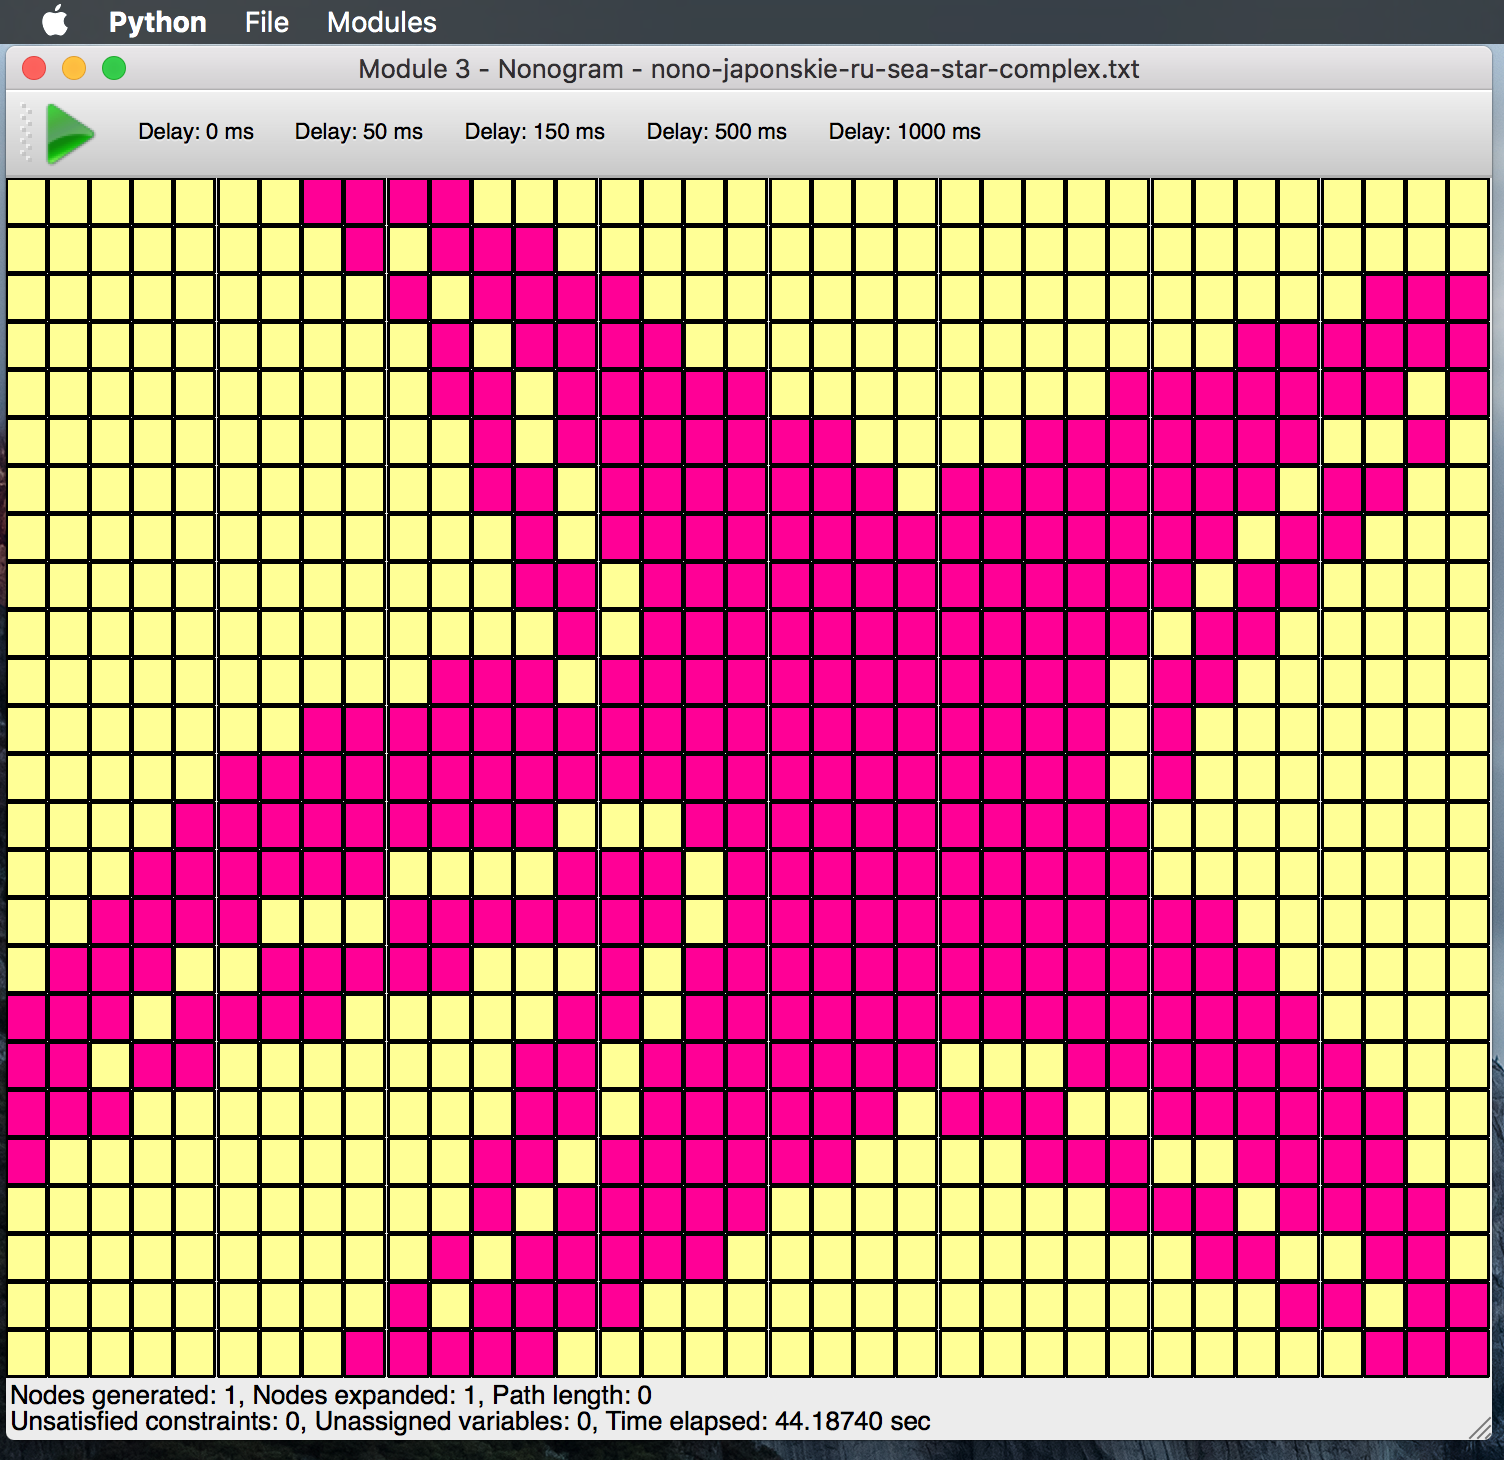
\includegraphics[width=0.5\textwidth]{module_3/images/nonogram}
  \caption{Solution to a nonogram found on en.japonskie.ru.}
  \label{constraint:vertex}
\end{figure}
